% !TeX root = ../main.tex
% Add the above to each chapter to make compiling the PDF easier in some editors.

\chapter{Congruence Closure with Explain Operation}\label{chapter:congruence_closure}

\section{Implementation}

For the implementation of the congruence closure algorithm, I followed the implementation described in the paper. \cite{Nieuwenhuis}

\subsection{Modified Union Find Algorithm}

In order to implement an explain operation with reasonble runtime for the congruene closure data structure, the paper \cite{Nieuwenhuis} introduced an alternative union find algorithm. The find algorithm remains the same, but a new data structure is introduced, called the proof forest, namely a forest which has as nodes the variables, and as edges the unions that were made. The forest structure is preserved, because redundant unions are ignored. 


\subsubsection{add\_edge}

The tree has directed edges, and for each equivalence class there is a representative node, where all the edges are directed towards. To keep this invariant, each time and edge from e to e' is added, all the edges on the path from the root of to e are reversed. 
In my implementation, the forest is represented by an array which stores the parent of each node, exactly as in the union find array. My implementation for each added edge is the following.

\begin{lstlisting}
function (domintros) add_edge :: "nat list => nat => nat => nat list"
where
"add_edge pf e e' = (if pf ! e = e 
			then (pf[e := e']) 
			else add_edge (pf[e := e']) (pf ! e) e)"
by pat_completeness auto
\end{lstlisting}

I was able to show that the \lstinline{add_edge e e'} terminates, if the \lstinline{ufa_invar} holds for the proof forest and $e$ and $e'$ do not belong to the same equivalence class. 

\begin{lstlisting}
lemma add_edge_domain: 
assumes "ufa_invar l" "rep_of l y != rep_of l y'"
shows "add_edge_dom (l, y, y')"
\end{lstlisting}


\begin{proof}
I proved it by induction on the length of the path p from the root of y to y. 
The base case is when there is only one node in the path, therefore y must be equal to its representative, therefore \lstinline{pf ! y = y}, and the algorithm terminates immediately.
On the other hand, if y is not a root, there is a path p' from the root to the parent of y which is shorter than the path from the root to y. Given that only the y is modified in the recursive step, and y is not on the path $p'$, the path p' is also present in the updated union find list. Also, the representative of y in the new list is equal to the representative of y', and the representative of the parent of y is still the old representative of y, therefore they are not in the same representative class, and we can apply the induction hypothesis and conclude that the recursive call terminates, therefore the function terminates.
\end{proof}



\tikzset{every picture/.style={line width=0.75pt}} %set default line width to 0.75pt        

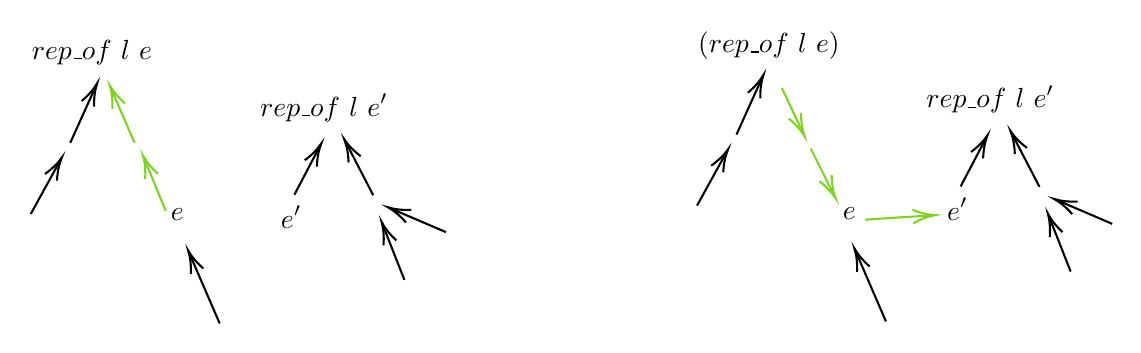
\begin{tikzpicture}[x=0.75pt,y=0.75pt,yscale=-1,xscale=1]
	%uncomment if require: \path (0,190); %set diagram left start at 0, and has height of 190
	
	%Straight Lines [id:da7388909588496015] 
	\draw [color={rgb, 255:red, 126; green, 211; blue, 33 }  ,draw opacity=1 ]   (86,78) -- (74.79,52.07) ;
	\draw [shift={(74,50.23)}, rotate = 66.63] [color={rgb, 255:red, 126; green, 211; blue, 33 }  ,draw opacity=1 ][line width=0.75]    (10.93,-3.29) .. controls (6.95,-1.4) and (3.31,-0.3) .. (0,0) .. controls (3.31,0.3) and (6.95,1.4) .. (10.93,3.29)   ;
	%Straight Lines [id:da932845693599931] 
	\draw [color={rgb, 255:red, 126; green, 211; blue, 33 }  ,draw opacity=1 ]   (101,110.77) -- (90.76,85.85) ;
	\draw [shift={(90,84)}, rotate = 67.66] [color={rgb, 255:red, 126; green, 211; blue, 33 }  ,draw opacity=1 ][line width=0.75]    (10.93,-3.29) .. controls (6.95,-1.4) and (3.31,-0.3) .. (0,0) .. controls (3.31,0.3) and (6.95,1.4) .. (10.93,3.29)   ;
	%Straight Lines [id:da8126326447235763] 
	\draw    (55,78) -- (67.18,51.05) ;
	\draw [shift={(68,49.23)}, rotate = 114.32] [color={rgb, 255:red, 0; green, 0; blue, 0 }  ][line width=0.75]    (10.93,-3.29) .. controls (6.95,-1.4) and (3.31,-0.3) .. (0,0) .. controls (3.31,0.3) and (6.95,1.4) .. (10.93,3.29)   ;
	%Straight Lines [id:da6899851051736223] 
	\draw    (36,112.23) -- (50.03,86.75) ;
	\draw [shift={(51,85)}, rotate = 118.85] [color={rgb, 255:red, 0; green, 0; blue, 0 }  ][line width=0.75]    (10.93,-3.29) .. controls (6.95,-1.4) and (3.31,-0.3) .. (0,0) .. controls (3.31,0.3) and (6.95,1.4) .. (10.93,3.29)   ;
	%Straight Lines [id:da19284936033329814] 
	\draw    (163,103) -- (175.07,80) ;
	\draw [shift={(176,78.23)}, rotate = 117.69] [color={rgb, 255:red, 0; green, 0; blue, 0 }  ][line width=0.75]    (10.93,-3.29) .. controls (6.95,-1.4) and (3.31,-0.3) .. (0,0) .. controls (3.31,0.3) and (6.95,1.4) .. (10.93,3.29)   ;
	%Straight Lines [id:da21247734751433156] 
	\draw    (201,103.23) -- (187.92,78) ;
	\draw [shift={(187,76.23)}, rotate = 62.59] [color={rgb, 255:red, 0; green, 0; blue, 0 }  ][line width=0.75]    (10.93,-3.29) .. controls (6.95,-1.4) and (3.31,-0.3) .. (0,0) .. controls (3.31,0.3) and (6.95,1.4) .. (10.93,3.29)   ;
	%Straight Lines [id:da18784825583709686] 
	\draw    (216,144) -- (205.73,117.86) ;
	\draw [shift={(205,116)}, rotate = 68.55] [color={rgb, 255:red, 0; green, 0; blue, 0 }  ][line width=0.75]    (10.93,-3.29) .. controls (6.95,-1.4) and (3.31,-0.3) .. (0,0) .. controls (3.31,0.3) and (6.95,1.4) .. (10.93,3.29)   ;
	%Straight Lines [id:da43419875667135477] 
	\draw    (236,121) -- (209.84,109.79) ;
	\draw [shift={(208,109)}, rotate = 23.2] [color={rgb, 255:red, 0; green, 0; blue, 0 }  ][line width=0.75]    (10.93,-3.29) .. controls (6.95,-1.4) and (3.31,-0.3) .. (0,0) .. controls (3.31,0.3) and (6.95,1.4) .. (10.93,3.29)   ;
	%Straight Lines [id:da8377415360718197] 
	\draw    (127,165) -- (112.59,131.64) ;
	\draw [shift={(111.8,129.8)}, rotate = 66.64] [color={rgb, 255:red, 0; green, 0; blue, 0 }  ][line width=0.75]    (10.93,-3.29) .. controls (6.95,-1.4) and (3.31,-0.3) .. (0,0) .. controls (3.31,0.3) and (6.95,1.4) .. (10.93,3.29)   ;
	%Straight Lines [id:da9212006749144803] 
	\draw [color={rgb, 255:red, 126; green, 211; blue, 33 }  ,draw opacity=1 ]   (397.86,51.57) -- (407.95,72.99) ;
	\draw [shift={(408.8,74.8)}, rotate = 244.78] [color={rgb, 255:red, 126; green, 211; blue, 33 }  ,draw opacity=1 ][line width=0.75]    (10.93,-3.29) .. controls (6.95,-1.4) and (3.31,-0.3) .. (0,0) .. controls (3.31,0.3) and (6.95,1.4) .. (10.93,3.29)   ;
	%Straight Lines [id:da9112225070236206] 
	\draw [color={rgb, 255:red, 126; green, 211; blue, 33 }  ,draw opacity=1 ]   (411.8,80.8) -- (422.91,103.01) ;
	\draw [shift={(423.8,104.8)}, rotate = 243.43] [color={rgb, 255:red, 126; green, 211; blue, 33 }  ,draw opacity=1 ][line width=0.75]    (10.93,-3.29) .. controls (6.95,-1.4) and (3.31,-0.3) .. (0,0) .. controls (3.31,0.3) and (6.95,1.4) .. (10.93,3.29)   ;
	%Straight Lines [id:da026589038011743282] 
	\draw    (376,74) -- (388.18,47.05) ;
	\draw [shift={(389,45.23)}, rotate = 114.32] [color={rgb, 255:red, 0; green, 0; blue, 0 }  ][line width=0.75]    (10.93,-3.29) .. controls (6.95,-1.4) and (3.31,-0.3) .. (0,0) .. controls (3.31,0.3) and (6.95,1.4) .. (10.93,3.29)   ;
	%Straight Lines [id:da4465748806717764] 
	\draw    (357,108.23) -- (371.03,82.75) ;
	\draw [shift={(372,81)}, rotate = 118.85] [color={rgb, 255:red, 0; green, 0; blue, 0 }  ][line width=0.75]    (10.93,-3.29) .. controls (6.95,-1.4) and (3.31,-0.3) .. (0,0) .. controls (3.31,0.3) and (6.95,1.4) .. (10.93,3.29)   ;
	%Straight Lines [id:da8556828124311282] 
	\draw    (484,99) -- (496.07,76) ;
	\draw [shift={(497,74.23)}, rotate = 117.69] [color={rgb, 255:red, 0; green, 0; blue, 0 }  ][line width=0.75]    (10.93,-3.29) .. controls (6.95,-1.4) and (3.31,-0.3) .. (0,0) .. controls (3.31,0.3) and (6.95,1.4) .. (10.93,3.29)   ;
	%Straight Lines [id:da17154675848466616] 
	\draw    (522,99.23) -- (508.92,74) ;
	\draw [shift={(508,72.23)}, rotate = 62.59] [color={rgb, 255:red, 0; green, 0; blue, 0 }  ][line width=0.75]    (10.93,-3.29) .. controls (6.95,-1.4) and (3.31,-0.3) .. (0,0) .. controls (3.31,0.3) and (6.95,1.4) .. (10.93,3.29)   ;
	%Straight Lines [id:da5166223592338979] 
	\draw    (537,140) -- (526.73,113.86) ;
	\draw [shift={(526,112)}, rotate = 68.55] [color={rgb, 255:red, 0; green, 0; blue, 0 }  ][line width=0.75]    (10.93,-3.29) .. controls (6.95,-1.4) and (3.31,-0.3) .. (0,0) .. controls (3.31,0.3) and (6.95,1.4) .. (10.93,3.29)   ;
	%Straight Lines [id:da8973818170227796] 
	\draw    (557,117) -- (530.84,105.79) ;
	\draw [shift={(529,105)}, rotate = 23.2] [color={rgb, 255:red, 0; green, 0; blue, 0 }  ][line width=0.75]    (10.93,-3.29) .. controls (6.95,-1.4) and (3.31,-0.3) .. (0,0) .. controls (3.31,0.3) and (6.95,1.4) .. (10.93,3.29)   ;
	%Straight Lines [id:da17526153342314021] 
	\draw [color={rgb, 255:red, 126; green, 211; blue, 33 }  ,draw opacity=1 ]   (438,115) -- (469.8,112.93) ;
	\draw [shift={(471.8,112.8)}, rotate = 176.28] [color={rgb, 255:red, 126; green, 211; blue, 33 }  ,draw opacity=1 ][line width=0.75]    (10.93,-3.29) .. controls (6.95,-1.4) and (3.31,-0.3) .. (0,0) .. controls (3.31,0.3) and (6.95,1.4) .. (10.93,3.29)   ;
	%Straight Lines [id:da07613740586925388] 
	\draw    (448,164) -- (433.59,130.64) ;
	\draw [shift={(432.8,128.8)}, rotate = 66.64] [color={rgb, 255:red, 0; green, 0; blue, 0 }  ][line width=0.75]    (10.93,-3.29) .. controls (6.95,-1.4) and (3.31,-0.3) .. (0,0) .. controls (3.31,0.3) and (6.95,1.4) .. (10.93,3.29)   ;
	
	% Text Node
	\draw (35,27) node [anchor=north west][inner sep=0.75pt]   [align=left] {$\displaystyle rep\_of\ l\ e$};
	% Text Node
	\draw (102,108) node [anchor=north west][inner sep=0.75pt]   [align=left] {$\displaystyle e$};
	% Text Node
	\draw (155,107) node [anchor=north west][inner sep=0.75pt]   [align=left] {$\displaystyle e'$};
	% Text Node
	\draw (145,53) node [anchor=north west][inner sep=0.75pt]   [align=left] {$\displaystyle rep\_of\ l\ e'$};
	% Text Node
	\draw (356,23) node [anchor=north west][inner sep=0.75pt]   [align=left] {$\displaystyle (rep\_of\ l\ e)$};
	% Text Node
	\draw (425.8,107.8) node [anchor=north west][inner sep=0.75pt]   [align=left] {$\displaystyle e$};
	% Text Node
	\draw (476,103) node [anchor=north west][inner sep=0.75pt]   [align=left] {$\displaystyle e'$};
	% Text Node
	\draw (466,49) node [anchor=north west][inner sep=0.75pt]   [align=left] {$\displaystyle rep\_of\ l\ e'$};
	
	
\end{tikzpicture}


\subsubsection{add\_label}

Additionally, each edge is labeled with the input equation or the input equations which caused the adding of this edge. This step is not necessaary for the union find algorithm by itself, but only for this algorithm when it is used within the congruence closure algorithm, because there are two possible reasons for the union of two elements a and b: either an equation $a = b$ was input, or two equations of the type $F(a_1, a_2) = a$ $F(b_1, b_2) = b$, where a1 and b1 bzw a2 and b2 were already in the same equivalence class before this union. Therefore we need to store the information about these input equations, in order to reconstruct the explanation in the end via the explain function. I implemented the labeling by using an additional list, which at each index contains the label of the outgoing edge, or \lstinline{None} if there is no outgoing edge. The type of the label is \lstinline{pending_equation}, which can be either \lstinline{One equation} or \lstinline{Two equation equation}, aka one or two equations. The name \lstinline{pending_equation} derived from the fact that they are also the elements of the pending list, which is going to be described in the next section. Theoretically this allows also for invalid equations for example two equations of the type $a = b$ and $c = d$, but we will prove in the next sections, that the equations in the labels list are always of a valid type.

Each time an edge, gets added to the proof forest, the labels need to be updated as well, not only the labels of the new edge, but also of the outgoing edges. The function which implements this is the following:

\begin{lstlisting}
function (domintros) add_label :: "pending_equation option list => nat list => nat 
=> pending_equation => pending_equation option list"
  where
"add_label pfl pf e lbl = (if pf ! e = e 
		then (pfl[e := Some lbl]) 
		else add_label (pfl[e := Some lbl]) pf (pf ! e) (the (pfl ! e)))"
by pat_completeness auto
\end{lstlisting}

Similarly to the \lstinline{path_to_root} function, \lstinline{add_label} has the same recursive calls/case distinctions as \lstinline{rep_of}, therefore it has the same domain.

\begin{lstlisting}
lemma rep_of_dom_iff_add_label_dom: "rep_of_dom (pf, y) <--> 
add_label_dom (pfl, pf, y, y')"
\end{lstlisting}


\subsection{Congruence Closure Data Structure}

\subsection{Congruence Closure Algorithm}

\section{Abstract Formalisation of Congruence Closure}

\section{Correctness Proof}

\section{Implementation of the Explain Operation}
